\documentclass[12pt]{article}
\usepackage{graphicx}
\usepackage{natbib}
\usepackage{url}
\usepackage{appendix}
\usepackage[british]{babel}
\usepackage{amsmath}


\bibpunct[:]{(}{)}{;}{a}{,}{,}

\renewcommand{\baselinestretch}{1.5}
\begin{document}
\begin{titlepage}

\begin{center}
{\Huge \bf Profitability of moving average trading strategies in the JSE top 40 share index. \vspace{1cm}

\Large Research Proposal} \vspace{1cm}

\today\\
Herman Claassens (student number: CLSHER003)
{\tt clsher003@myuct.ac.za}

\end{center}
\end{titlepage}

\tableofcontents
\newpage

\section{Introduction}
Technical analysis and moving average trading systems have been widely used by financial market practitioners. A study by (Gunasekaragea and Power, 2001) suggested that technical rules could be used in emerging markets to provided excess returns when compared to a simple buy-and-hold strategy. Can a moving average trading rule be used to generate such returns in a South African context? The proposal will outline the key research question, methodologies and literature that will be consulted when attempting to answer this question. Furthermore, it will give a  time-scale for both the planning and execution of the proposed research project. 

\pagenumbering{arabic}

\section{Background to research}
\label{sec:background}

Various trading strategies fall under the broad term of technical analysis. A technical analyst studies past prices in the hope of correctly predicting future prices. Technical analysis dates back to the 1800s and was widely used in the period prior to extensive disclosure of financial information. Although many early studies regarding technical analysis have concluded that it is useless, more recently it has undergone a renaissance (Brock, Lakonishok and LeBaron, 1992). Sweeney (1988) showed that filter trading rules can outperform the market. A popular tool among technical analysts is moving averages, which is a smoothing mechanism to view trends in time series data. Moving averages help analysts devise a strategy for buying and selling stocks. 

\section{Problem statement}
\label{sec:prob state}
The research will answer the following question: 
\\Do moving average trading strategies generate excess returns when compared to a basic buy-and-hold strategy in the JSE top 40 Index once transaction costs have been taken into account.

\subsection{Other key research questions}
\label{sub:other key quest} 
The research will subsequently also touch on the following:
\begin{enumerate}
\item Is the South African stock market weak form efficient?
\item Which moving average leads to the highest returns?

\end{enumerate}

\section{Literature review}
\label{sec:lit rev}

The efficient market hypothesis states that share prices fully incorporate all relevant information. In it's weak form, the information set is restricted to only past price history (Fama, 1970). Consequently, if we accept weak form efficiency, technical analysts would not be able to profit from analysing past share prices. The research would thus also have an impact on our understanding of the efficiency of the South African investment environment. Important work regarding market effeciency has been done by Malkiel (2003). This will be a important source of literature when discussing the efficient market hypothesis. 

In its most basic of forms, a moving average is defined as the sum of a number of closing stock prices over a given period, divided by the number of periods. Moving averages smooth out a time series and reduces the noise in a series, allowing one to identify the trend in prices. There are a wide range of different types of moving averages, all with different advantages and disadvantages for identifying market movement. Consider two moving averages, one with a short period and another with a longer period. These moving averages generate buy(sell) signals when the shorter moving average penetrates the longer moving average from below(above) (Sobreiro et all, 2016). The moving averages do not, however, give any indication as to how long the upward or downward trend will persist (James, 1968). The work of James (1968) will be consulted when evaluating the effectiveness of moving averages as trading strategies. 

Brock, Lakonishok and LeBaron (1992) found that simple trading rules had predictive powers when applied to the Dow Jones Index between the years 1897 and 1986. Hudson et all (1996) did a similar study and found that when such simple trading rules are applied to the Financial Times Industrial Ordinary Index from 1935 to 1994, they also appear to have predictive ability. However, both these studies concluded that when transaction costs are to be taken into account, these simple trading rules are unlikely to outperform a simple buy-and-hold strategy. More recently, Sobreiro et all (2016) found that in some emerging markets there are periods where a moving average trading rule outperforms the passive strategy. This study was limited by the fact that it did not take into account any transaction costs on the simulated trades. The proposed research will use moving averages to simulates buy/sell signals in the JSE Top 40 Index while also taking into account transaction costs. In the South African context, transaction costs on share trades amount to the following:
\begin{itemize}
\item Brokerage fees
\item Investor protection levy
\item STRATE settlement charge
\item Securities transfer tax
\end{itemize} 
In our project, trading costs will be a fixed percentage of the entire trade value. We will be taking trading costs into account at both a 5\% and 2\% level. 

\section{Methodology}
\label{sec:meth}

The proposed research will test five moving averages in the Top 40 Index over a period of five years. The different moving averages (MA's) are listed below:

\begin{itemize}
\item Simple moving average (SMA)
\item Exponential moving average (EMA)
\item Weighted moving average (WMA)
\item Volume weighted moving average (VWMA)
\item Triple exponential moving average (TEMA)
\end{itemize} 
Each of the listed MA's will have a short period and a long period. In order to avoid a situation where we fit MA models to our index data until we find a scenario where our trading strategy outperforms the buy-and-hold strategy; we divide our five year period of interest into a optimisation period of three years and a two year out-of-sample test period. We use the optimisation period to find pseudo optimal short and long periods for each MA. These 'optimal' periods are then tested in the out-of-sample test period to evaluate their performance against the buy-and-hold strategy.

Firstly, we start by choosing a short and long period that is widely used by industry practitioners. For each MA, we plot the short and long MA on our Top 40 time series. When the short MA cuts the long MA from below, a buy signal is generated and we will assume that the total index will be bought. The index will be held until a sell signal is generated when the short MA cuts the long MA from above. The entire index will then be sold. The log-returns of our holding periods can them be determined: 
\begin{equation}
r_i=log(P_{S_i}/P_{B_i})
\end{equation}
Where: \\

$r_i$ is the return in the $i$th holding period

$P_{S_i}$ is the index value at the time of a sell signal for holding period $i$

$P_{B_i}$ is the index value at the time of a buy signal for holding period $i$

$log$ is the natural logarithm.\\
\noindent\\
Thus we end up with the log-returns over the entire optimisation period. The total log-return over the entire optimisation period can then be calculated as follows: 
\begin{equation}
R_{MA} = \sum_{j=1}^{n} r_i
\end{equation} 
Where:\\

$R_{MA}$ is the total log return for moving average MA over the

optimisation period

$n$ is the total number of holding periods

$r_i$ is the return in the $i$th holding period\\
\noindent\\
The summation above is possible due to the fact that log returns are time additive. 

Under the buy-and-hold strategy the full index will be held from the outset until the end of the optimisation period. The log-return over this period can easily be calculated by using (1) above. 

By comparing the return on the buy-and-hold strategy to our given MA trading strategy we can evaluate whether or not excess returns have been generated. 

We now repeat the process a number of times, changing the long period for our MA of interest at the outset of each iteration and keeping the short period constant. These iterations help us find a pseudo optimal long period for each of our MA's i.e. the long period that ensured the highest total return over the optimisation period. Once we have found our appropriate long period we then find a 'optimal' short period by applying the same procedure but by fixing the long period of our specific MA to its 'optimal' level, as calculated earlier. 

Our chosen periods for each MA is then applied to our out of sample test period. The log-returns over this period is compared to that of the buy-and-hold strategy over the same period in order to establish whether or not any of our MA's have generated excess returns and if so, which MA lead to the highest returns. 

\section{Timeline }

This section will outline significant milestones and important dates w.r.t the research project (see figure 1). 

An next important aspect of the research project will be the literature review. The review must by submitted by 16:00 on Monday the 12th of June. After this proposal has been submitted there will be 33 full days before our literature review is due. It would be ideal to have the content of the review completed plus minus a week before submission. This will leave us with enough time to format and spell check our document. It will also ensure that enough time is spent on compiling the reference list and double checking the referencing. 

The next important milestone would be the submission of the draft paper on the 11th of September at 12:00. This leaves us with 91 days between the submission of our literature review and our draft submission. After consulting with our supervisor, it was determined that the most complex and time consuming aspect of our project would be writing the R code for our trading strategy simulations. Five moving averages have to be tested by using the methodology set out above. This will thus be our main focus after the literature review has been submitted. Once we have coded and executed the simulations for one of our moving averages, the other four should merely be extensions of what we have already done. We will complete the simulations for our first moving average no later than the  2nd of July. We will then complete the testing of the rest of our moving averages over a period of about a month. Leaving us with enough time to do our write-up and draw conclusions. 

Once our draft has been submitted, it will be evaluated and we will be given feedback. It will then be crucial to identify areas in the project that needs attention according to the feedback. Once these areas have been identified, we can set up a timeline for how to correct any problem areas. The final paper will be submitted on the 6th of November at 16:00. 

\begin{figure}
  \caption{Research project timeline.}
  \centering
    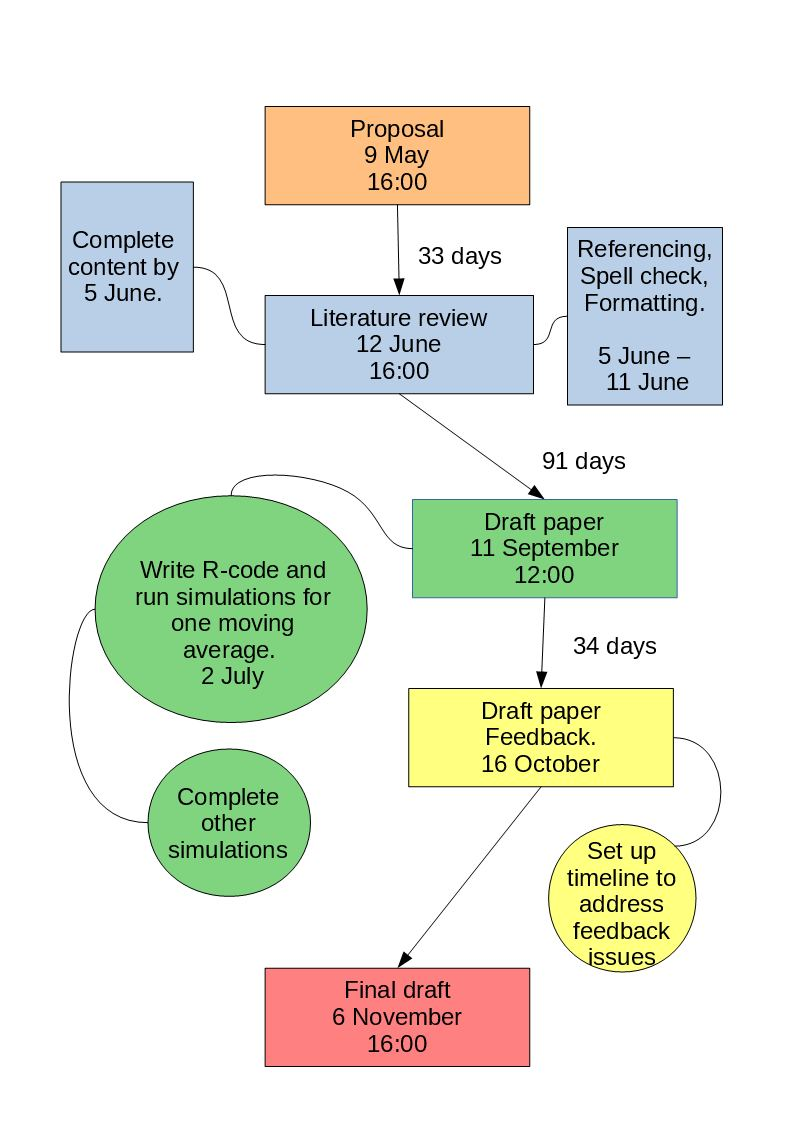
\includegraphics[width=1\textwidth]{timeline_final}
\end{figure}


\section{Importance of research}
The findings of the research will be of importance to both investors who are actively trading shares on the JSE or those who are merely holding a well diversified portfolio. If the research shows that our trading strategy generates access returns, passive investors would be better off by employing our identified strategy. 

As previously mentioned, the paper will also serve as evidence as to whether or not the South African stock market is weak form efficient. If no excess returns are generated, we will be able to conclude that the market is in fact weak form efficient. If this is the case, an argument can be made against institutional investors.  

\section{Structure of paper}
The proposed structure of the paper:
\begin{enumerate}
\item Introduction
\item Background to research
\item Summary of literature review
\item Methodology and data
\item Results
\item Discussion 
\item Conclusion
\item References
\item Appendices

\end{enumerate}
\newpage
\section{References}

\noindent
Brock, W. Lakonishok, J. and LeBaron, B. 1992. Simple Technical Trading Rules and the Stochastic Properties of Stock Returns. \textit{The Journal of Finance.} 47(5): 1731-1764. DOI: 10.2307/2328994.
\\
\\
Fama, E.F. 1970. Efficient Capital Markets: A Review of Theory and Empirical Work. \textit{The Journal of Finance.} 25(2): 28-30. DOI: 10.2307/2325486. 
\\
\\
Gunasekarage, A. Power, D.M. 2001. The profitability of moving average trading rules in South Asian stock markets. \textit{Emerging Markets Review}. 2(1): 17-33. DOI: https://doi.org/10.1016/S1566-0141(00)00017-0.
\\
\\
James, F.E. 1968. Monthly Moving Averages--An Effective Investment Tool? \textit{The Journal of Financial and Quantitative Analysis.} 3(2): 315-326. DOI: 10.2307/2329816. 
\\
\\
Malkiel, B.G. 2003. The Efficient Market Hypothesis and Its Critics. \textit{The Journal of Economic Perspectives.} 17(1):  59-82.  Available: http://www.jstor.org/stable/3216840 [2017, April 30].
\\
\\
Sobreiro, V.A. da Costa, T.R.C.C. Nazário, R.T.F. e Silva, J.L. Moreira, E.A. Lima Filho, M.C. Kimura, H. and Zambrano, J.C.A. 2016. The profitability of moving average trading rules in BRICS and emerging stock markets. \textit{The North American Journal of Economics and Finance.} 38: 86-101. DOI: https://doi.org/10.1016/j.najef.2016.08.003
\\
\\
Sweeney, R.J. 1988. Some New Filter Rule Tests: Methods and Results. \textit{The Journal of Financial and Quantitative Analysis.} 23(3): 285-300. DOI: 10.2307/2331068.







\end{document}










